% 2019-01-28

\documentclass[10pt]{article}
\usepackage[T1]{fontenc}
\usepackage{amssymb}
\usepackage{amsmath}
\usepackage{graphicx}
% \begin{figure}[h]
% \centering
% \includegraphics[width=6.5in]{folder/photo.png}
% \caption{}
% \label{}
% \end{figure}



\usepackage{tikz}
\usetikzlibrary{arrows}
\usepackage{subfigure}
\usepackage{stackrel}
\usepackage{blindtext}

\usepackage[url=false]{biblatex}
\addbibresource{library.bib}

\oddsidemargin=0.15in
\evensidemargin=0.15in
\topmargin=-.5in
\textheight=9in
\textwidth=6.25in

\usepackage[colorlinks=true,breaklinks,pdfpagemode=none,linkcolor=blue,citecolor=blue]{hyperref}

\usepackage{enumerate}
% \vspace{-6pt}
% \begin{itemize}
%     \setlength{\itemsep}{0pt}%
%     \setlength{\parskip}{0pt}%
%     \item Item 1
%     \item Item 2
%         \begin{itemize}
%             \setlength{\itemsep}{0pt}%
%             \setlength{\parskip}{0pt}%
%             \item Sublist Item 1
%             \item Sublist Item 2
%         \end{itemize}
%         \item Item 3
% \end{itemize}
% \vspace{-6pt}


\usepackage{enumitem}
\setlist{itemsep=0mm}

\usepackage{amsmath,amsfonts,amssymb,bm}


\begin{document}

   \noindent
   \begin{center}

   \hrulefill
   
   \vspace{5pt}
   
   \makebox[\textwidth]{ {\bf Energy Systems Analysis} \hfill  A.D. Smith 2019}
   \vspace{0pt}
   
   {\Large \hfill  Lecture 8. Building Energy Modeling (BEM): Building and Weather Files}
   \vspace{5pt}
   
  
   \hrulefill
   \end{center}


{\color{darkgray}{\color{darkgray}{\center{ \small{      ``Model utility depends not on whether its driving scenarios are realistic (since no one can know that for sure), but on whether it responds with a realistic pattern of behavior.''
\\%[3pt]
\rightline{{\rm --- Donella H. Meadows \cite{meadows}}}}}}}}

\section{Building files}

An EnergyPlus main input file is a human-readable text file with the suffix \textbf{\textit{.idf} (for Input Data File)}. It describes the characteristics of the building, its HVAC system, and its surroundings to a limited extent. This information is the basis for the implementation of equations representing the physics in the simulation, but does not provide a 3-D representation of how everything is arranged. 

% EnergyPlus has a standard set of SI units that are internally used for calculations, although you can ask for output in IP units. Depending on the interface you use, you may be able to enter your data in IP units as well.

The most straightforward, least glamorous way to interact with an IDF file is through the IDF Editor (Figure \ref{IDFeditor}), ``a simple, `intelligent' editor that reads the EnergyPlus Data Dictionary (IDD) and allows creation/revision of EnergyPlus Input Files.'' \cite{EP9docs} The IDF Editor is accessed through the EP Launch program (Figure \ref{EPlaunch}), only available for the Windows Platform.

            \begin{figure}[h]
            \centering
            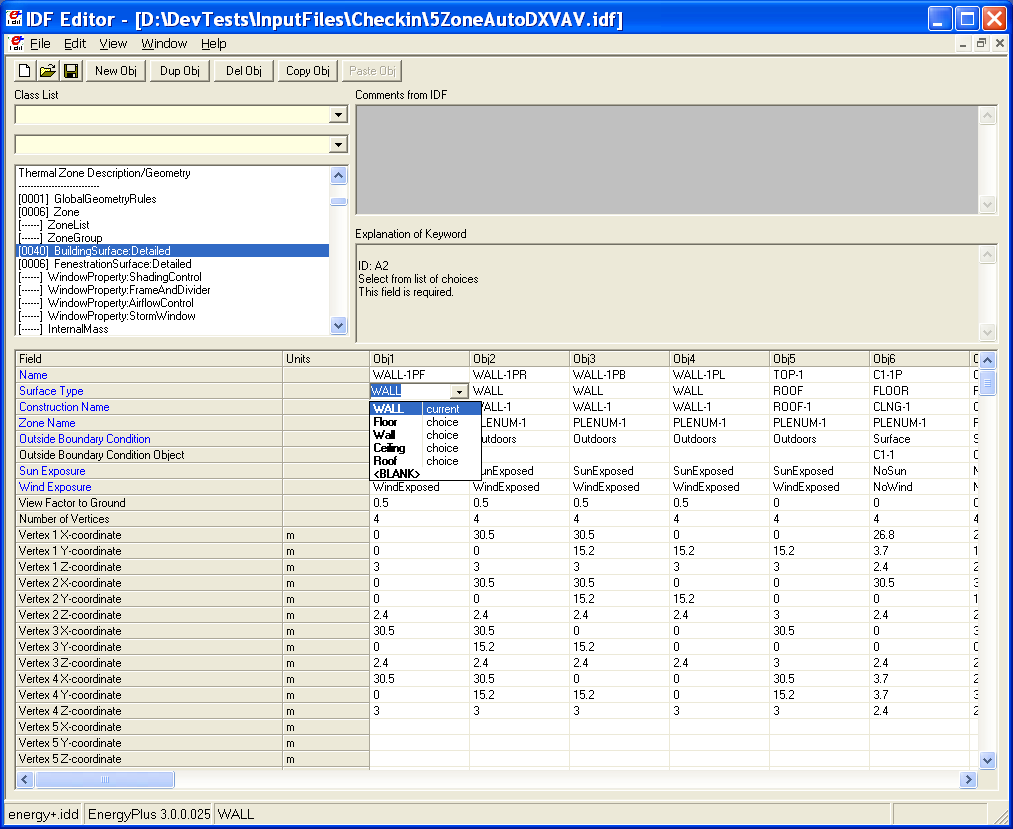
\includegraphics[width=5in]{extras08/IDFediting.png}
            \caption{IDF Editor in action \cite{EP9docs}}
            \label{IDFeditor}
            \end{figure}


 You can also open the IDF with any text editor as it is simply a standard ASCII text file, and most interfaces built on the EnergyPlus engine will just modify the IDF behind the scenes according to your commands. Each item within the IDF file that has data associated with it is called an \textbf{object}.  A group of related objects forms a \textbf{class}. Comments follow exclamation points. 

The \textbf{Input Data Dictionary (IDD)} is a file that tells EnergyPlus what is allowable and what to expect with the IDF file it will be reading. Refer to ``IDD Conventions'' in the Input-Output Reference document \cite{EP9docs} for a description of what the IDD should look like. Although it is a critical input file, we will not modify the IDD files in our class, instead using existing IDD files and working within the structure they provide for how we present data to the EnergyPlus engine. 

For a given simulation, the two key input files we will focus on will be IDF and EPW files, described in the next section. We will stop to take a look at the contents of the IDF files as we learn to run simulations over the next couple of weeks. Even if you don't directly modify the IDF file in practice, it will help your understanding of the EnergyPlus BEM process for you to discover their typical structure, and try to decipher what inputs are affecting what simulation outcomes based on what EnergyPlus is actually reading from the input files.

            \begin{figure}[h]
            \centering
            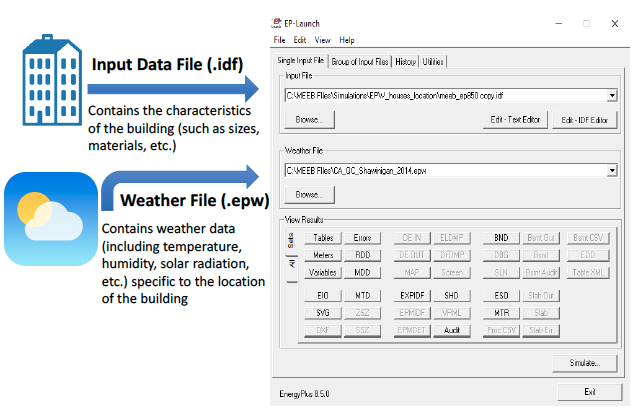
\includegraphics[width=5in]{extras08/EPinterface.png}
            \caption{EP Launch Program \cite{Bianchi-dissertation}}
            \label{EPlaunch}
            \end{figure}




\section{Weather files}

A weather file tells the software what the simulated building will ``experience'' throughout the simulation. This assumes that the weather is uniform around the building---not always a great assumption, and one that my research team and collaborators are helping to evaluate quantitatively. If you've had heat transfer, this means that the dry bulb temperature provided by the weather file would be your $T_\infty$. 

An EnergyPlus weather file is a human-readable csv text file with the suffix \textbf{\textit{.epw} (for EnergyPlus Weather)}. The top of the file contains headers, site information, design conditions, and some information about holidays and daylight savings time. It contains weather data over a period of time (usually 1 year) at intervals of at least one hour (although higher-resolution data can be included). 


The following variables are included:
\begin{itemize}
    \setlength{\itemsep}{0pt}%
    \setlength{\parskip}{0pt}%
    \item Dry Bulb Temperature
    \item Dew Point Temperature
    \item  Relative Humidity
    \item  Atmospheric Station Pressure
    \item 6 fields of radiation data
    \item 4 fields of illuminance data
    \item Wind Direction
    \item  Wind Speed
    \item 4 fields relating to cloud cover and visibility
    \item 6 fields relating to precipitation
\end{itemize}

Refer to EnergyPlus documentation, Auxiliary Programs section for details \cite{EP9docs}.

\subsection{Impact of weather on building energy use}

Some buildings are more 'weather driven' than others, for reasons you might guess, such as: 
\begin{itemize}
    \setlength{\itemsep}{0pt}%
    \setlength{\parskip}{0pt}%
    \item high \textbf{skin ratio} (surface area-to-volume ratio for the building envelope),
    \item high \textbf{window-to-wall ratio},
    \item low insulation values (small U values),
    \item instances of \textbf{thermal bridging} (easy pathways for heat transfer between conditioned space and the outdoors),
    \item \textbf{natural ventilation} (i.e. not mechanically forced) or high rates of \textbf{outdoor air} as opposed to recirculating air,
    \item or simply having low indoor loads (e.g. low plug loads, low occupant density)
\end{itemize}

The types of HVAC systems that condition the building and their efficiencies and maintenance schedules will also affect how much a building is affected by hot, cold, or changing weather conditions outside. There is also simulation-based evidence that buildings in cold climates are more affected by weather than those in warm climates \cite{Hong2013-ti}.

\subsection{Typical Meteorological Years}

The \textbf{typical meteorological year (TMY)} is a conceptual ``representative'' weather year for a given location. 

\begin{quote}
To calculate a TMY, a multiyear data set is analyzed and 12 months are chosen from that time frame that best represent typical conditions. \cite{tmy-nsrdb}
\end{quote}

The TMY files are designed to illustrate what a building's performance might be, on average, in a certain climate. While they are compiled using statistical techniques starting with actual observed weather data, they don't represent any given consecutive yearlong period in historical time. By definition, they don't capture unusual weather patterns, which leads to an important cautionary note:

\begin{quote}
Because TMYs represent typical rather than extreme conditions, they are not suited for designing systems to meet the worst-case conditions occurring at a location. \cite{tmy-nsrdb}
\end{quote}

A TMY file is not necessarily provided in EPW format, as TMY files do exist for other applications. We will download EPW files from the EnergyPlus website \cite{EPweather}, which are TMY weather data in the form of EPW files, ready for use in EnergyPlus building energy simulations. You may see options for TMY, TMY2 or TMY3 data. TMY3 data sets are the most recent, derived from 1991--2005 weather, and provide more geographic locations than previous TMY versions \cite{TMY3user}.  TMY2 data sets are less recent, based on  1961--1990 weather \cite{TMY2user}, but still widely used.  The original TMY data sets were produced using 1952--1975 weather \cite{TMY3user}. TMY3 will be our preferred type of TMY data.

It's also important to note that the observed data usually come from the airport nearest to the named city, which may not be well correlated with the weather data in the urban center \cite{Carlo1}. Take a look at weather observations from DarkSky \cite{DarkSky} or MesoWest \cite{MesoWest} right now--can you find a downtown station and one at SLC airport? How different are their readings?

\subsection{Actual Meteorological Years}

An \textbf{actual meteorological year (AMY)} is simply the actual weather detected in a given place during a historical year. For building model \textbf{calibration}, which involves comparing model output to actual performance data, an AMY weather file is necessary. There are companies that sell AMY files using historical weather data that has been processed into the EPW format \cite{noauthor_undated-vj}. We also now have an open source solution, described below.

\subsubsection{Localized AMY File Creator (LAF)}

NREL engineer and former Site-Specific Energy Systems Lab researcher Dr. Carlo Bianchi created a weather file converter to take MesoWest \cite{MesoWest} observed weather data and present it in the EnergyPlus--friendly EPW format, ready for use in EnergyPlus building energy simulations. This software is our first release of the weather file creator.

Download and install the LAF app for your platform at \url{https://energysystems.mech.utah.edu/laf/}. You can also grab the Python code directly at \url{https://github.com/sseslab/laf/}.  We're working on the next version of LAF and your feedback is appreciated.

% license
\bigskip

\noindent
\texttt{\footnotesize RESTRICTED PUBLIC LICENSE --- READ BEFORE SHARING. This is a draft version made available by Amanda D. Smith under a Creative Commons Attribution-NonCommercial-ShareAlike license. 
\href{https://creativecommons.org/licenses/by-nc-sa/4.0/}{CC BY-NC-SA 4.0}}

% references

\printbibliography

\end{document}

